\section{Measurement Setup}
\label{sec:measurement_setup}

To research the influence of different initial window size on TCP and the
network, we chose the network virtualization framework Mininet~\cite{mininet}.
Mininet exploits existing os virtualization and resource management features of
the Linux kernel, namely Network namespaces~\cite{network_namespaces} and
Cgroups~\cite{cgroups}, to simulate multiple networks and peers on a single
host. Because no virtual machines are involved and Linux can make advantage of
zero-copy mechanism, the overhead of these Network namespaces is low. It can
easily simulate 10GbE-Networks using commodity PC-Hardware. Mininet also
integrates other features such as traffic control and OpenFlow, so one can build
arbitrary network topologies and conditions. To create and configure networks
Mininet exposes a Python API and allow to interact with network namespaces at
runtime by giving shell access.

\newcommand{\FixedScale}{0.7}

\begin{figure*}
\begin{tikzpicture}[
  start chain=going right,
  diagram item/.style={
    on chain,
    join
  },
  node distance=1cm and 3cm,
  scale=0.8, every node/.style={transform shape}
]

\node [
  diagram item,
  label=below:{Server (Nginx)}
] (server) {
\includegraphics[scale=\FixedScale]{figure/server_w_pc_router}};

\node [
  diagram item,
  label=center:{Internet}
] (internet) {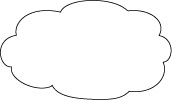
\includegraphics[scale=\FixedScale]{figure/cloud}};

\node [
  diagram item,
  label=below:Modem/Router
] (router) {
\includegraphics[scale=\FixedScale]{figure/cable_modem}};

\node [
  diagram item,
  label=below:{Client (cURL)}
] (client) {
\includegraphics[scale=\FixedScale]{figure/pc}};

\draw (server)   -- (internet);
\draw (internet) -- (router) node[pos=0.62,text width=3cm] {BW: variable,\\Delay: variable};
\draw (router)   -- (client) node[pos=0.62,text width=3cm] {BW: 1Gbps,\\Delay: 1ms};
\end{tikzpicture}
\caption{Network Topology simulated using Mininet}
\end{figure*}


